\documentclass{article}
\usepackage{amsmath}
\usepackage{amsfonts}
\usepackage{amssymb}
\usepackage{cancel}

\usepackage{graphicx}


\setlength\parindent{0pt}

\author{Pranav Tikkawar}
\title{Workshop 4: 292}

\begin{document}
\maketitle
\begin{enumerate}
    \item - \begin{enumerate}
        \item [a] \begin{itemize}
            \item 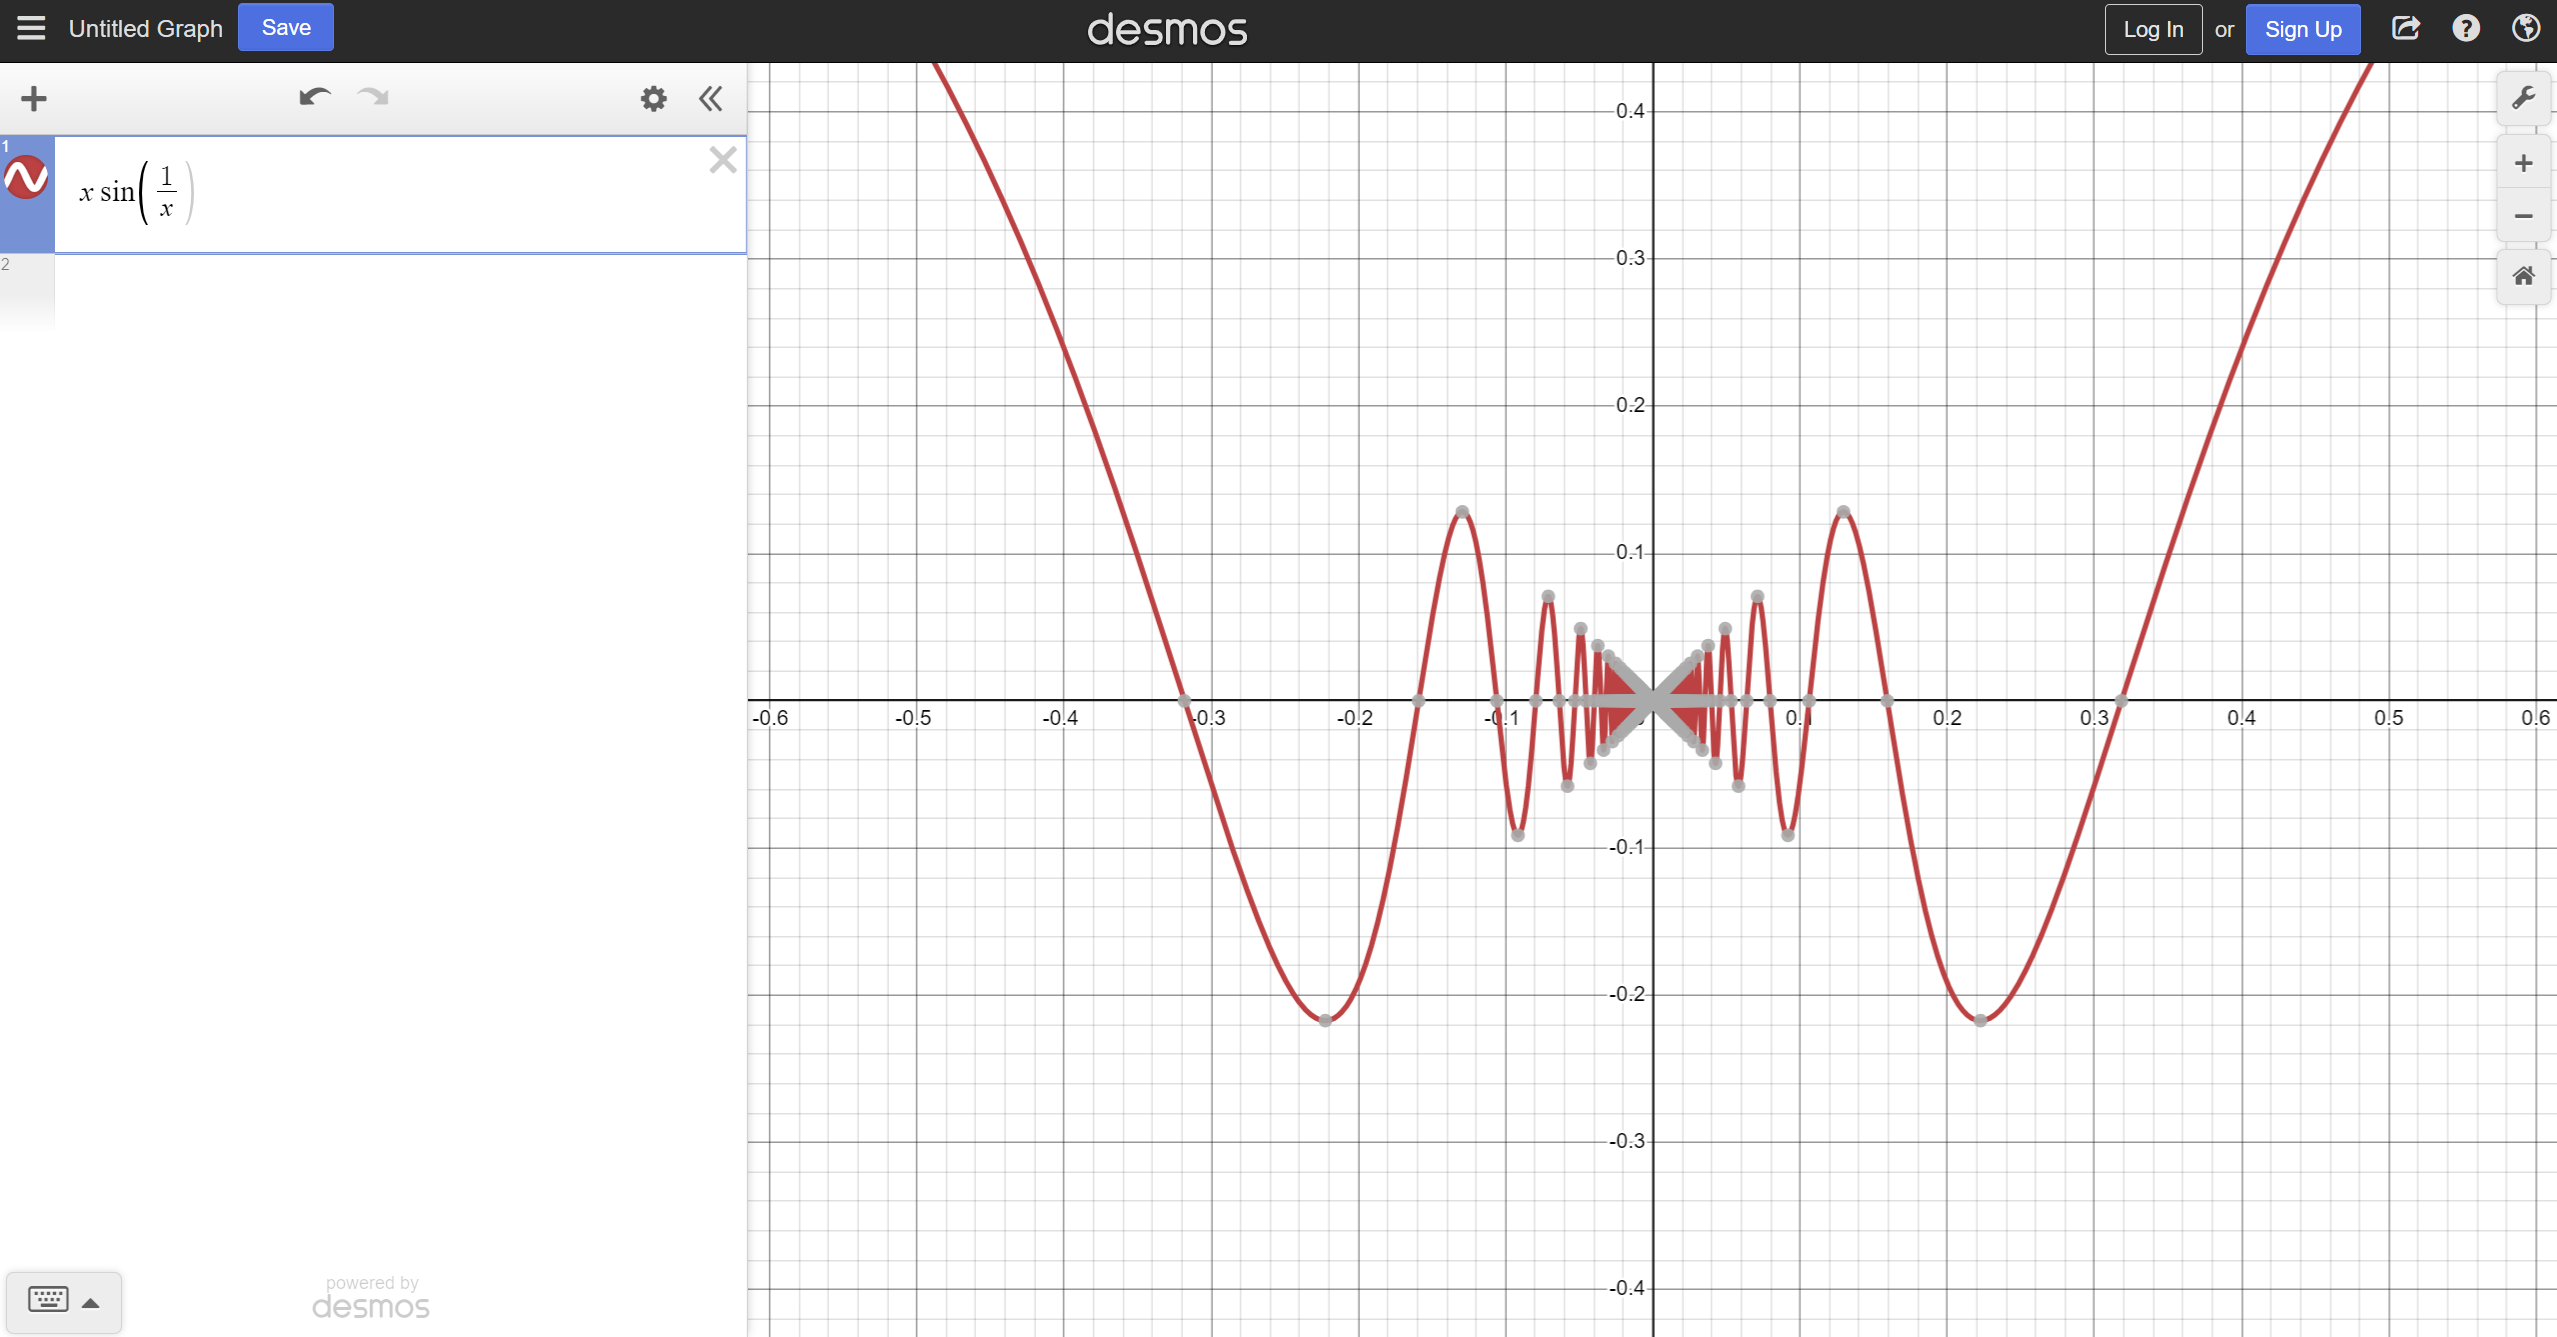
\includegraphics[scale=.2]{xsin.png}
        \end{itemize}
        \item [b] \begin{itemize}
            \item Since we need to use squeeze theorum to show what the limit of $v(x)$ by bounding it by 2 other functions and show the limit of those function approach the same thing at zero
            \item We can notice that $|v(x)| = |xsin(\frac{1}{x})| = |x| |sin(\frac{1}{x})|$
            \item The values of $|sin(\frac{1}{x})|$ are $0 \leq |sin(\frac{1}{x})| \leq 1$ and $|x|$ are $0 \leq |x| \leq |x| $ so $0 \leq |xsin(\frac{1}{x})| \leq |x|$
            \item We can notice than $\lim_{x \rightarrow 0} 0 = 0 $ and $\lim_{x \rightarrow 0} |x| = 0 $ so then $\lim_{x \rightarrow 0} |xsin(\frac{1}{x})|  = 0 $
        \end{itemize}
        \item [c] \begin{itemize}
            \item The most obvious EQ sol of the DE is $x = 0$ as $v(0)=0$
            \item If $x \neq 0 $ then $v(x) = xsin(\frac{1}{x})$
            \item If we want $v(x) = 0$ then we need $sin(\frac{1}{x}) = 0$
            \item Since $sin(y) = 0$ if $y = n\pi$ where $n \in \mathbb{Z} $
            \item So $ x = \frac{1}{n\pi}$
        \end{itemize}
        \item [d] \begin{itemize}
            \item There are many maximum intervals but it is important to recognize that as they approach 0 the intvervals become more and more dense
            \item Let $n \in \mathbb{Z} $ the max intervals for $n>0$ is $(\frac{1}{(n+1)\pi}, \frac{1}{n\pi}) $. It represents all the max intervals for $x>0$. Also we need to consider the interval $(\frac{1}{\pi},\infty) $
            \item The max intervals for $n<0$ is $(\frac{1}{(n)\pi}, \frac{1}{(n+1)\pi}) $ this represents the max intervals for $x<0$. Also we need to consider the interval $(-\infty,\frac{-1}{\pi})$
        \end{itemize}
        \item [e] \begin{itemize}
            \item Since we know $xsin(1/x)$ is periodic we know that one we find the sign of the $v(x)$ of one interval then we can deduce the rest.
            \item * look at image*
        \end{itemize}
        \item [f] \begin{itemize}
            \item $\frac{|v(y_n) - v(x_n)|}{|y_n - x_n|}$ will provide an $ L$ to test if v is Lipschitz continuous on R, but using the given $x_n$ and $y_n$ we get the ratio = $4n$ 
            \item As $\lim_{n \rightarrow \infty} 4n = \infty$ which means that $v(x)$ is not Lipschitz on the interval as for every L we can choose to be the bounding ratio, we choose and n that beats it
        \end{itemize}
        \item [g]\begin{itemize}
            \item To find the maximum interval we need to show that $|v'(x)|$ is bounded by $L$ 
            \item $|v'(x)| = |sin(\frac{1}{x}) - \frac{1}{x}cos(\frac{1}{x})|\leq |sin(\frac{1}{x})| + |\frac{1}{x}||cos(\frac{1}{x})| $ due to the triangle inequality
            \item Since $0 \leq |sin(\frac{1}{x})| \leq 1 $ and $0 \leq |cos(\frac{1}{x})| \leq 1 $ and we can suppose an $a$ s.t. $|x| > a > 0$ we get $|v'(x)| \leq 1 + \frac{1}{a}$ 
            \item Which gives $L = 1 + \frac{1}{a}$ which indicates that since $L neq \infty $ then the function $v(x)$ is continuous on that interval
        \end{itemize}
        \item [h] \begin{itemize}
            \item If we suppose an $\epsilon \in \mathbb{R}$ where $(0,\epsilon)$ is the maximum interval, we can find a number smaller than epsilon such that it is a equilibrium point as in the formula for equilibrium points shown above, as n increase the equilibrum points become more dense around 0. Thus making this a contradiction
            \item Since it is a contradiction and we know that going from one maximum interval to the other in the function, it must change direction, we can see that $x(t) = 0 $ is the unique solution to $x(t_0) = 0 $
        \end{itemize}
        \item [i] \begin{itemize}
            \item $\infty$ for $x_0 > \frac{1}{x}$  
            \item $0$ for $x_0 = 0$
            \item $\frac{1}{n\pi} = \frac{1}{n\pi} $
            \item $\frac{1}{(2n) \pi} $ for $\frac{1}{(2n+1)\pi} < x_0 < \frac{1}{(2n -1)\pi} $
            \item $ \infty $ for $x_0 < \frac{-1}{\pi}$: 
        \end{itemize}
    \end{enumerate}
\end{enumerate}

\end{document}